\clearpage
\subsection{premi/client/presentationManager}
%diagramma del package%
\begin{figure}[h]
\begin{center}
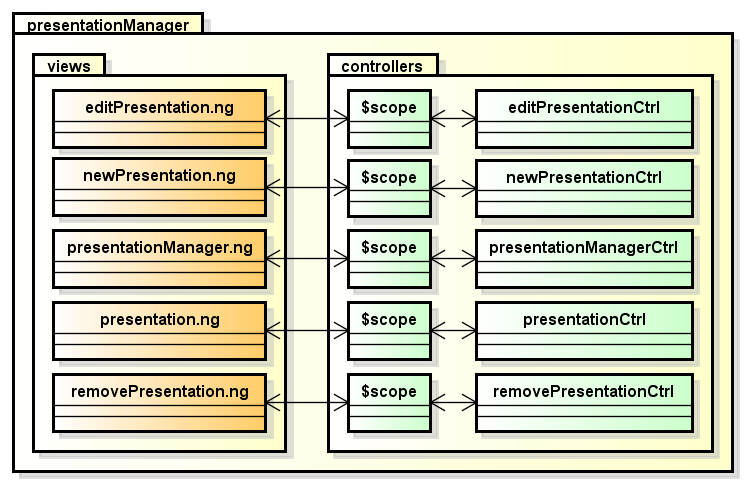
\includegraphics[scale=0.50]{img/diapkg/presentationManager.png}
\caption{Diagramma del package premi/client/presentationManager}
\end{center}
\end{figure}











%-------  diagramma di un template %
\subsubsection{premi/client/presentationManager/views/editPresentation.ng}

\begin{description}
%-------  descrizione del template%
\item[Descrizione] \hfill
	Template della vista associata allo \textit{\$scope} di \textit{editPresentationCtrl}. Permette all'utente di modificare titolo e descrizione di una presentazione.
\item[Note] \hfill
	\begin{itemize}
			\item Mostra il titolo della presentazione in un input HTML$_G$, modificabile, attraverso l'attributo dello \textit{\$scope} Presentation.title
			\item Mostra la descrizione della presentazione in un input HTML$_G$, modificabile, attraverso l'attributo dello scope Presentation.description
			\item Possiede un bottone associato al metodo \textit{save()} dello \textit{\$scope} per salvare la presentazione
			\item Possiede un bottone associato al metodo \textit{discard()} dello \textit{\$scope} per annullare le modifiche effettuate sulla presentazione
	\end{itemize}
\end{description}

%-------  diagramma di un template %
\subsubsection{premi/client/presentationManager/views/newPresentation.ng}

\begin{description}
%-------  descrizione del template%
\item[Descrizione] \hfill
	Template della vista associata allo \textit{\$scope} di \textit{newPresentationCtrl}. Permette all'utente di creare una nuova presentazione, fornendo un titolo e una descrizione.
\item[Note] \hfill
	\begin{itemize}
			\item Mostra un input HTML nel quale inserire il titolo della presentazione, che va associato all'attributo \textit{title} dello \textit{\$scope}
			\item Mostra un input HTML nel quale inserire la descrizione della presentazione, che va associata all'attributo \textit{description} dello \textit{\$scope}
			\item Possiede un bottone associato al metodo \textit{save()} dello \textit{\$scope} per salvare la presentazione
			\item Possiede un bottone associato al metodo \textit{discard()} dello \textit{\$scope} per annullare la creazione della presentazione
	\end{itemize}
\end{description}

%-------  diagramma di un template %
\subsubsection{premi/client/presentationManager/views/presentationManager.ng}

\begin{description}
%-------  descrizione del template%
\item[Descrizione] \hfill
	Template della vista associata allo \textit{\$scope} di \textit{presentationmagerCtrl}. Fornisce uno scheletro per le altre viste dedicate alla gestione delle presentazioni
\end{description}



%-------  diagramma di un template %
\subsubsection{premi/client/presentationManager/views/presentations.ng}

\begin{description}
%-------  descrizione del template%
\item[Descrizione] \hfill
	Template della vista associata allo \textit{\$scope} di \textit{presentationsCtrl}. Mostra una lista di tutte le presentazioni dell'utente
\item[Note] \hfill
	\begin{itemize}
			\item Mostra la lista delle presentazioni, le quali sono contenute nell'attributo \textit{Presentations} dello \textit{\$scope}
			\item Per ogni presentazione fornisce dei link per sua la modifica e rimozione
	\end{itemize}
\end{description}



%-------  diagramma di un template %
\subsubsection{premi/client/presentationManager/views/removePresentation.ng}

\begin{description}
%-------  descrizione del template%
\item[Descrizione] \hfill
	Template della vista associata allo \textit{\$scope} di \textit{removePresentationCtrl}. Permette all'utente di rimuovere una presentazione dal database.
\item[Note] \hfill
	\begin{itemize}
			\item Mostra un messaggio di conferma prima di rimuovere la presentazione
			\item Dopo il messaggio di conferma mostra un tasto associato al metodo \textit{remove()} dello \textit{\$scope} per la rimozione definitiva della presentazione
			\item Dopo il messaggio di conferma mostra un tasto associato al metodo \textit{discard()} dello \textit{\$scope} per annullare il processo di rimozione della presentazione
	\end{itemize}
\end{description}





























%-------  diagramma della classe%
\subsubsection{premi/client/presentationManager/controllers/editPresentationCtrl}
\begin{figure}[h]
\begin{center}
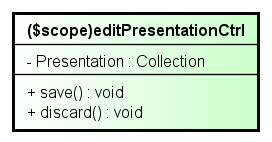
\includegraphics[scale=0.90]{img/diacla/editPresentationCtrl.png}
\caption{Diagramma della classe premi/client/presentationManager/controllers/editPresentationCtrl}
\end{center}
\end{figure}

\begin{description}
%-------  descrizione della classe%
\item[Descrizione] \hfill
	Controller della view \textit{editPresentation.ng}. Permette all'utente di modificare titolo e descrizione di una presentazione.
	

%-------  lista delle classi associate%	
\item[Associazioni] \hfill
	\begin{itemize}
		\item \textbf{client/presentation/lib/databaseAPI}: per salvare la presentazione modificata
	\end{itemize}

	
%-------  lista degli Attributi%	
\item[Attributi] \hfill
	\begin{description}
		\item[\textbf{+ Presentation : Collection			}] \hfill
			Presentazione che l'utente intende modificare. Viene inizializzata dal controller tramite il codice identificativo passato come parametro dal browser (servizio \$stateParams di AngularJS)
	\end{description}
	
	
%-------  lista dei metodi%	
\item[Metodi] \hfill

	% -- inizio metodo -- %
	\begin{description}
		\item[\textbf{\color{blue}+ save() : void			}] \hfill
			Utilizza il metodo \textit{+ updatePresentation(id, title, description)} di databaseAPI per il salvataggio della presentazione nel database. Rimanda poi alla lista delle presentazioni utilizzando l'oggetto \textit{\$state} di \textit{\$stateProvider}
	\end{description}
	% -- fine metodo -- %		
	
	% -- inizio metodo -- %
	\begin{description}
		\item[\textbf{\color{blue}+ discard() : void			}] \hfill
			Annulla le modifiche effettuate dall'utente sul titolo e sulla descrizione della presentazione. Rimanda poi alla lista delle presentazioni utilizzando l'oggetto \textit{\$state} di \textit{\$stateProvider}
	\end{description}
	% -- fine metodo -- %	
	
	
	
\end{description}

%-------  diagramma della classe%
\subsubsection{premi/client/presentationManager/controllers/newPresentationCtrl}
\begin{figure}[h]
\begin{center}
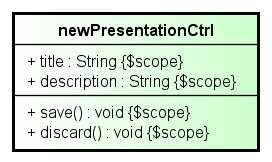
\includegraphics[scale=0.90]{img/diacla/newPresentationCtrl.png}
\caption{Diagramma della classe premi/client/presentationManager/controllers/newPresentationCtrl}
\end{center}
\end{figure}




\begin{description}
%-------  descrizione della classe%
\item[Descrizione] \hfill
	Controller della view \textit{newPresentation.ng}. Permette all'utente di creare una nuova presentazione e di salvarla nel database.
	

%-------  lista delle classi associate%	
\item[Associazioni] \hfill
	\begin{itemize}
		\item \textbf{client/presentation/lib/databaseAPI}: per salvare la presentazione nel database
	\end{itemize}

	
%-------  lista degli Attributi%	
\item[Attributi] \hfill
	\begin{description}
		\item[\textbf{+ title : String			}] \hfill
		Il titolo della nuova presentazione
		\item[\textbf{+ description : String			}] \hfill	
		La descrizione della nuova presentazione
	\end{description}
	
	
%-------  lista dei metodi%	
\item[Metodi] \hfill

	% -- inizio metodo -- %
	\begin{description}
		\item[\textbf{\color{blue}+ save() : void			}] \hfill
			Utilizza il metodo \textit{+ insertNewPresentation(title, description)} di databaseAPI per il salvataggio della presentazione nel database. Rimanda poi alla lista delle presentazioni utilizzando l'oggetto \textit{\$state} di \textit{\$stateProvider}
	\end{description}
	% -- fine metodo -- %		
	
	% -- inizio metodo -- %
	\begin{description}
		\item[\textbf{\color{blue}+ discard() : void			}] \hfill
			Annulla le modifiche effettuate dall'utente sul titolo e sulla descrizione della presentazione. Rimanda poi alla lista delle presentazioni utilizzando l'oggetto \textit{\$state} di \textit{\$stateProvider}
	\end{description}
	% -- fine metodo -- %	
	
	
	
\end{description}




%-------  diagramma della classe%
\subsubsection{premi/client/presentationManager/controllers/presentationManagerCtrl}
\begin{figure}[h]
\begin{center}
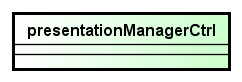
\includegraphics[scale=0.90]{img/diacla/presentationManagerCtrl.png}
\caption{Diagramma della classe premi/client/presentationManager/controllers/presentationManagerCtrl}
\end{center}
\end{figure}

\begin{description}
%-------  descrizione della classe%
\item[Descrizione] \hfill
	Questo controller non è al momento provvisto di funzionalità. Si appoggia alla vista associata \textit{presentationManager.ng}, la quale funge da scheletro per le viste necessarie alla gestione delle presentazioni dell'utente.
\end{description}




%-------  diagramma della classe%
\subsubsection{premi/client/presentationManager/controllers/presentationsCtrl}
\begin{figure}[h]
\begin{center}
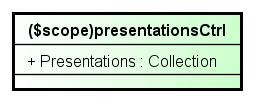
\includegraphics[scale=0.90]{img/diacla/presentationsCtrl.png}
\caption{Diagramma della classe premi/client/presentationManager/controllers/presentationsCtrl}
\end{center}
\end{figure}

\begin{description}
%-------  descrizione della classe%
\item[Descrizione] \hfill
	Fornisce alla vista associata \textit{presentations.ng} una lista di tutte le presentazioni in possesso dell'utente
	
	
%-------  lista degli Attributi%	
\item[Attributi] \hfill
	\begin{description}
		\item[\textbf{+ Presentations : Collection			}] \hfill
			Collezione MongoDB di presentazioni. Viene inizializzata dal controller prelevando le presentazioni pubblicate al client.
	\end{description}

\end{description}





%-------  diagramma della classe%
\subsubsection{premi/client/presentationManager/controllers/removePresentationCtrl}
\begin{figure}[h]
\begin{center}
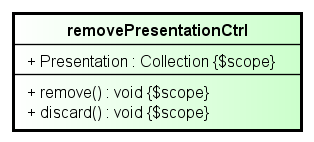
\includegraphics[scale=0.90]{img/diacla/removePresentationCtrl.png}
\caption{Diagramma della classe premi/client/presentationManager/controllers/removePresentationCtrl}
\end{center}
\end{figure}




\begin{description}
%-------  descrizione della classe%
\item[Descrizione] \hfill
	Controller della view \textit{removePresentation.ng}. Permette all'utente di eliminare una presentazione da lui creata in precedenza.
	

%-------  lista delle classi associate%	
\item[Associazioni] \hfill
	\begin{itemize}
		\item \textbf{client/presentation/lib/databaseAPI}: per effettuare la rimozione sul database
	\end{itemize}

	
%-------  lista degli Attributi%	
\item[Attributi] \hfill
	\begin{description}
		\item[\textbf{+ Presentation : Collection			}] \hfill
			Presentazione che l'utente intende rimuovere. Viene inizializzata dal controller tramite il codice identificativo passato come parametro dal browser (servizio \$stateParams di AngularJS)
	\end{description}
	
	
%-------  lista dei metodi%	
\item[Metodi] \hfill

	% -- inizio metodo -- %
	\begin{description}
		\item[\textbf{\color{blue}+ remove() : void			}] \hfill
			Utilizza il metodo \textit{+ removePresentation(id, title, description)} di databaseAPI per la rimozione della presentazione dal database. Rimanda poi alla lista delle presentazioni utilizzando l'oggetto \textit{\$state} di \textit{\$stateProvider}
	\end{description}
	% -- fine metodo -- %		
	
	% -- inizio metodo -- %
	\begin{description}
		\item[\textbf{\color{blue}+ discard() : void			}] \hfill
			Annulla le modifiche effettuate dall'utente sulla presentazione. Rimanda poi alla lista delle presentazioni utilizzando l'oggetto \textit{\$state} di \textit{\$stateProvider}
	\end{description}
	% -- fine metodo -- %	
	
	
	
\end{description}















